Функция \texttt{count\_common\_roads} в C++ использует \texttt{передачу аргументов по ссылке} в целях эффективности. Это не влияет на то, как вы должны вызывать процедуру.
Гарантируется, что проверяющий модуль не меняет значения в $r$.

\texttt{find\_roads(4, [0, 0, 0, 1, 1, 2], [1, 2, 3, 2, 3, 3])}


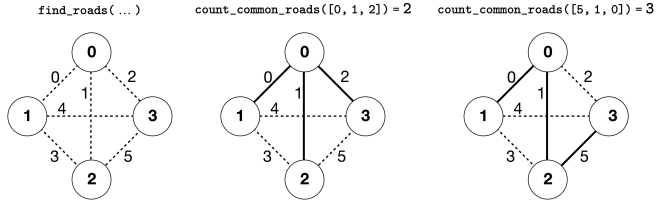
\includegraphics[scale=0.7]{1.png}

В данном примере есть $4$ города и $6$ дорог. Обозначим за $(a, b)$ дорогу, соединяющую города $a$ и $b$. Дороги пронумерованы от $0$ до $5$ в следующем порядке: $(0, 1)$, $(0, 2)$, $(0, 3)$, $(1, 2)$, $(1, 3)$, и $(2, 3)$. Каждый набор золотых дорог содержит ровно $n - 1 = 3$ дорог.

Предположим, что шахскими являются дороги $0$, $1$ и $5$, то есть, дороги $(0, 1)$, $(0, 2)$ и $(2, 3)$, а программа совершает следующие вызовы:

\begin{itemize}
\item \texttt{count\_common\_roads([0, 1, 2])} который возвращает $2$. В данном запросе
рассматриваются дороги с номерами $0, 1$, и $2$, то есть, дороги $(0, 1)$, $(0, 2)$ и $(0,3)$. Две из них являются шахскими.
\item \texttt{count\_common\_roads([5, 1, 0])} который возвращает $3$. В данном запросе
рассматриваются все дороги, принадлежащие шахскому набору дорог.
\end{itemize}

Функция \texttt{find\_roads} должна вернуть $[5, 1, 0]$ или любой другой массив длины $3$, который содержит три данных элемента.

Обратите внимание, что следующие вызовы не являются допустимыми.
\begin{itemize}
\item \texttt{count\_common\_roads([0, 1])}: длина массива $r$ не равна $3$.
\item \texttt{count\_common\_roads([0, 1, 3])}: массив $r$ не описывает золотой набор дорог, так как невозможно добраться из города $0$ в город $3$, используя только дороги $(0,1)$, $(0,2)$, $(1,2)$.
\end{itemize}